\section{Experiments}
\label{sec:experiments}

\subsection{Experimental setup}
\label{sec:setup}

\paragraph{Base models and tools.}
We use Qwen3-VL-Thinking~\citep{Qwen3VL} at three sizes (2B, 4B, 8B) as the base model across all methods. The tool set is the three families introduced in \autoref{sec:prelim-rl}: a Python interpreter, a web search engine (Tavily search API\footnote{https://www.tavily.com/}), and an image zoom-in tool. 
All tools share a unified \texttt{<tool\_call>} interface. Full prompt templates and tool schemas are in \appref{app:tools}.

\paragraph{Training data \& pipeline.}
SFT uses 64K correct trajectories drawn from ViRL~\citep{virl}, fvqa~\citep{fvqa}, and PyVision-RL~\citep{pyvision-rl}, generated by Qwen3-VL-32B-Thinking~\citep{Qwen3VL} where $\sim$25\% contain a tool call. RL uses a 16K filtered subset plus 22K questions from MMFineReason-hard~\citep{mmfinereason}.
We follow the SFT then RL pipeline of \autoref{sec:prelim-rl}. AXPO augments the rollout loop with \toolresample, holding all other hyperparameters constant against SFT\,+\,GRPO. Full details are in \appref{app:training-setup}.

\paragraph{Benchmarks and metrics.}
We evaluate on nine multimodal benchmarks grouped into three task categories: \textbf{Reasoning} (MathVision~\citep{mathvision}, DynaMath~\citep{dynamath}, Math-VR~\citep{mathvr}), \textbf{Perception} (V$^{\star}$~\citep{vstar}, VisualProbe~\citep{mini-o3}, HR-Bench-4K and HR-Bench-8K~\citep{HRBench}), and \textbf{Search} (HR-MMSearch~\citep{hrmmsearch}, MMSearch~\citep{mmsearch}); per-benchmark descriptions in \appref{app:benchmarks}. All benchmarks are evaluated in the agentic setting with the same tool interface used in training. We report Pass@1 and Pass@4 (\%), averaged over four rollouts per question, with answer matching logic tailored for each benchmark.

\paragraph{Baselines.}
We compare AXPO against four baselines: (1) \textbf{Base}: the base model only with prompting without additional training (2) \textbf{SFT}: the SFT checkpoint without RL (3) \textbf{GRPO}: RL from the base model without an SFT stage and (4) \textbf{SFT\,+\,GRPO}: the standard SFT-then-RL recipe.
Our method, \textbf{SFT\,+\,AXPO}: applies \toolresample and advantage calculation from~\autoref{sec:method} on top of the same SFT-then-RL pipeline.

\subsection{Main Results: AXPO narrows the agentic gap to a 4$\times$ larger baseline.}
\label{sec:main-results}
\begin{table*}[t]
    \caption{Main results --- Pass@1 (\%, $\uparrow$) on \textbf{nine multimodal benchmarks}, grouped into three categories: Reasoning, Perception, and Search. All methods use \textbf{Qwen3-VL-Thinking}~\citep{Qwen3VL} at four sizes (2B, 4B, 8B, 32B). Best result per column within each size block is \textbf{bolded}; second-best is \underline{underlined}. \textit{$\Delta$} rows show AXPO's gain over SFT\,+\,GRPO, the strongest comparable training recipe where AXPO outperforms it in most of evaluations. Pass@4 results are reported in \autoref{tab:main-p4}.}
    \vspace{-0.1in}
    \label{tab:main-p1}
    \centering
    \small
    \resizebox{\textwidth}{!}{
    \begin{tabular}{l ccc cccc cc >{\columncolor{mygray}}c}
        \toprule
        \multicolumn{1}{c}{} &
        \multicolumn{3}{c}{\textbf{Reasoning}} &
        \multicolumn{4}{c}{\textbf{Perception}} &
        \multicolumn{2}{c}{\textbf{Search}} &
        \multicolumn{1}{c}{\multirow{2}{*}[-3pt]{\textbf{Avg.}}} \\
        \cmidrule(lr){2-4} \cmidrule(lr){5-8} \cmidrule(lr){9-10}
        \textbf{Method} &
        \shortstack{Math\\Vision} & \shortstack{Dyna\\Math} & \shortstack{Math\\-VR} &
        V$^{\star}$ & \shortstack{Visual\\Probe} & \shortstack{HRBen.\\-4K} & \shortstack{HRBen.\\-8K} &
        \shortstack{HR-MM\\Search} & \shortstack{MM\\Search} & \multicolumn{1}{c}{} \\
        \midrule

        \multicolumn{11}{l}{\textit{Qwen3-VL-2B-Thinking}} \\
        \midrule
        Base
            & 18.6 & 60.5 & 16.9 & 63.0 & 5.0 & 64.6 & 55.9 & 8.2 & 27.7 & 35.6 \\
        GRPO
            & 33.7 & 64.9 & 34.6 & 67.1 & 23.8 & 65.0 & 59.4 & \textbf{18.4} & \textbf{41.4} & 45.4 \\
        SFT
            & 28.9 & 64.1 & 30.2 & 75.9 & 24.5 & 73.1 & 68.8 & 14.5 & 35.9 & 46.2 \\
        \quad+\,GRPO
            & \underline{34.8} & \underline{66.4} & \underline{35.8} & \textbf{81.7} & \textbf{36.1} & \underline{74.3} & \underline{70.6} & 15.7 & \underline{40.6} & \underline{50.7} \\
        \rowcolor{myblue}
        \quad+\,\textbf{AXPO}\,\scalebox{0.8}{\textit{(Ours)}}
            & \textbf{35.0} & \textbf{66.9} & \textbf{38.9} & \underline{81.3} & \underline{35.1} & \textbf{77.9} & \textbf{72.4} & \underline{18.1} & 40.3 & \textbf{51.8} \\
        \rowcolor{myblue!50}
        \textit{\;\;$\Delta$ vs.\ SFT\,+\,GRPO}
            & \dpos{0.2} & \dpos{0.5} & \dpos{3.1} & \dneg{0.4} & \dneg{1.0} & \dpos{3.6} & \dpos{1.8} & \dpos{2.4} & \dneg{0.3} & \dposavg{1.1} \\
        \midrule

        \multicolumn{11}{l}{\textit{Qwen3-VL-4B-Thinking}} \\
        \midrule
        Base
            & 48.0 & \underline{76.6} & 50.8 & 80.6 & 24.8 & 73.6 & 67.5 & 16.9 & 37.8 & 53.0 \\
        GRPO
            & \underline{52.5} & 76.2 & \textbf{57.9} & 82.7 & 29.7 & 75.5 & 71.1 & 12.7 & 23.8 & 53.6 \\
        SFT
            & 49.1 & 76.3 & 55.3 & 87.0 & 34.7 & \underline{79.5} & \underline{74.1} & \textbf{20.6} & 41.5 & 57.6 \\
        \quad+\,GRPO
            & 51.6 & \textbf{77.2} & \underline{57.4} & \textbf{90.2} & \underline{38.0} & 78.8 & 73.8 & 20.0 & \underline{42.3} & \underline{58.8} \\
        \rowcolor{myblue}
        \quad+\,\textbf{AXPO}\,\scalebox{0.8}{\textit{(Ours)}}
            & \textbf{52.8} & 76.4 & 57.2 & \underline{88.9} & \textbf{43.6} & \textbf{80.9} & \textbf{78.3} & \underline{20.1} & \textbf{43.3} & \textbf{60.2} \\
        \rowcolor{myblue!50}
        \textit{\;\;$\Delta$ vs.\ SFT\,+\,GRPO}
            & \dpos{1.2} & \dneg{0.8} & \dneg{0.2} & \dneg{1.3} & \dpos{5.6} & \dpos{2.1} & \dpos{4.5} & \dpos{0.1} & \dpos{1.0} & \dposavg{1.4} \\
        \midrule

        \multicolumn{11}{l}{\textit{Qwen3-VL-8B-Thinking}} \\
        \midrule
        Base
            & 47.1 & 75.9 & 54.9 & 77.7 & 31.8 & 72.8 & 66.1 & 21.0 & 42.7 & 54.4 \\
        GRPO
            & 54.4 & 77.2 & 58.9 & 85.7 & \underline{40.1} & 77.1 & 73.9 & 20.6 & \textbf{45.1} & 59.2 \\
        SFT
            & 50.9 & 76.8 & 58.4 & 84.8 & 38.4 & \underline{79.5} & 74.4 & 23.0 & 40.6 & 58.5 \\
        \quad+\,GRPO
            & \underline{55.3} & \underline{78.2} & \underline{60.4} & \underline{87.7} & \underline{40.1} & \underline{79.5} & \underline{74.9} & \underline{24.4} & 44.0 & \underline{60.5} \\
        \rowcolor{myblue}
        \quad+\,\textbf{AXPO}\,\scalebox{0.8}{\textit{(Ours)}}
            & \textbf{56.1} & \textbf{79.0} & \textbf{60.6} & \textbf{87.8} & \textbf{45.8} & \textbf{83.3} & \textbf{77.0} & \textbf{25.9} & \underline{45.0} & \textbf{62.3} \\
        \rowcolor{myblue!50}
        \textit{\;\;$\Delta$ vs.\ SFT\,+\,GRPO}
            & \dpos{0.8} & \dpos{0.8} & \dpos{0.2} & \dpos{0.1} & \dpos{5.7} & \dpos{3.8} & \dpos{2.1} & \dpos{1.5} & \dpos{1.0} & \dposavg{1.8} \\
        \midrule

        \multicolumn{11}{l}{\textit{Qwen3-VL-32B-Thinking} (inference-only baseline)} \\
        \midrule
        Base
            & 56.5 & 83.3 & 64.1 & 89.1 & 40.3 & 85.3 & 78.9 & 22.8 & 46.1 & 62.9 \\

        \bottomrule
    \end{tabular}
    }
\vspace{-0.15in}
\end{table*}



\autoref{tab:main-p1} reports Pass@1 across nine benchmarks at four model sizes (per-benchmark Pass@4 results in \autoref{tab:main-p4}, \appref{app:pass4-table}). SFT\,+\,AXPO outperforms SFT\,+\,GRPO at average performance on Pass@1 (\dPassOneTwoB{} / \dPassOneFourB{} / \dPassOneEightB\,pp at 2B/4B/8B). On Pass@4, SFT\,+\,AXPO also beats SFT\,+\,GRPO at every scale (\dPassFourTwoB{} / \dPassFourFourB{} / \dPassFourEightB\,pp). \textbf{At 8B, SFT\,+\,AXPO reaches \eightBPassOneReachPct{} of the 32B Base's Pass@1 and surpasses it on Pass@4 (\eightBvsAgentPassFour), despite having $4\times$ fewer parameters}. AXPO is the only recipe whose 8B point reaches the 32B line on Pass@1, and the only one whose Pass@4 crosses it (\autoref{fig:main}).

Decomposing the 8B Pass@1 column of \autoref{tab:main-p1}, SFT\,+\,AXPO gains \dReasoningEightB\,pp on Reasoning, \dPerceptionEightB\,pp on Perception, and \dSearchEightB\,pp on Search over the SFT\,+\,GRPO baseline.
In relative terms, the gain concentrates in Perception ($+4\%$) and is smallest on Reasoning ($+1\%$). Perception is where image-tool use most directly determines correctness, while on Reasoning the bottleneck is often the thinking rather than the tool call.
A detailed discussion of the results is provided in~\appref{app:decomp-recipe}.


\subsection{Ablations: All components of AXPO matter}
\label{sec:ablations}

\autoref{tab:ablation} ablates each AXPO design choice on 8B. Every component contributes: removing prefix fixing, the resampling target, uncertainty-based prefix selection, prefix credit, or the per-prefix advantage group all degrade both Pass@1 and Pass@4 average. Per-row analysis is in~\appref{app:ablation-details}.

\subsection{AXPO outperforms alternative RL recipes}
\label{sec:comparison}
\begin{table*}[t]
    \caption{\textbf{AXPO ablations} on \textbf{Qwen3-VL-8B-Thinking}. Each row removes (or alters) one AXPO design choice from the full method. All rows share the SFT initialization. Best per column is \textbf{bolded}; second-best \underline{underlined}.}
    \vspace{-0.1in}
    \label{tab:ablation}
    \centering
    \small
    \resizebox{\textwidth}{!}{
    \begin{tabular}{l cc cc cc cc >{\columncolor{mygray}}c>{\columncolor{mygray}}c}
        \toprule
        \textbf{Method} &
        \multicolumn{2}{c}{MathVision} &
        \multicolumn{2}{c}{V$^{\star}$} &
        \multicolumn{2}{c}{VisualProbe} &
        \multicolumn{2}{c}{HR-MMSearch} &
        \multicolumn{2}{c}{\textbf{Average}} \\
        \cmidrule(lr){2-3} \cmidrule(lr){4-5} \cmidrule(lr){6-7} \cmidrule(lr){8-9} \cmidrule(lr){10-11}
        SFT + & P@1 & P@4 & P@1 & P@4 & P@1 & P@4 & P@1 & P@4 & \multicolumn{1}{c}{P@1} & \multicolumn{1}{c}{P@4} \\
        \midrule

        AXPO\,w/o prefix fix (rollout from scratch)
            & 56.0 & 75.0 & 86.9 & \textbf{96.9} & 43.6 & \textbf{68.9} & \underline{21.9} & 35.7 & \underline{52.1} & \underline{69.1} \\
        \phantom{AXPO\,}w/\phantom{o} no-tool rollout resampling
            & 54.9 & 71.4 & \textbf{89.1} & \underline{96.3} & 41.5 & 62.3 & 21.1 & 33.4 & 51.7 & 65.9 \\
        \phantom{AXPO\,}w/o uncertainty rank
            & 53.0 & 72.4 & 85.7 & 93.2 & \underline{43.9} & 63.2 & 21.4 & 34.4 & 51.0 & 65.8 \\
        \phantom{AXPO\,}w/o prefix credit
            & \underline{57.2} & \textbf{76.6} & 86.3 & 95.3 & 40.6 & 62.3 & 21.6 & \underline{36.7} & 51.4 & 67.7 \\
        \phantom{AXPO\,}w/o separated advantage group
            & \textbf{57.7} & \textbf{76.6} & 87.2 & 95.8 & 40.1 & 61.3 & 19.8 & 34.4 & 51.2 & 67.0 \\
        \midrule
        \rowcolor{myblue}
        \textbf{AXPO}\,\scalebox{0.8}{\textit{(Ours)}}
            & 56.1 & \underline{75.7} & \underline{87.8} & 95.3 & \textbf{45.8} & \underline{67.9} & \textbf{25.9} & \textbf{42.0} & \textbf{53.9} & \textbf{70.2} \\

        \bottomrule
    \end{tabular}
    }
\end{table*}

\begin{table*}[t]
    \caption{\textbf{Comparison to alternative RL recipes} on \textbf{Qwen3-VL-8B-Thinking}. All rows share the SFT initialization. \textit{Reward shaping \& sampling} adds a per-tool-call reward or doubles the GRPO rollout budget. \textit{RL algorithms} replaces GRPO with another alternative. Best per column is \textbf{bolded}; second-best \underline{underlined}.}
    \vspace{-0.1in}
    \label{tab:comparison}
    \centering
    \small
    \resizebox{\textwidth}{!}{
    \begin{tabular}{l cc cc cc cc >{\columncolor{mygray}}c>{\columncolor{mygray}}c}
        \toprule
        \textbf{Method} &
        \multicolumn{2}{c}{MathVision} &
        \multicolumn{2}{c}{V$^{\star}$} &
        \multicolumn{2}{c}{VisualProbe} &
        \multicolumn{2}{c}{HR-MMSearch} &
        \multicolumn{2}{c}{\textbf{Average}} \\
        \cmidrule(lr){2-3} \cmidrule(lr){4-5} \cmidrule(lr){6-7} \cmidrule(lr){8-9} \cmidrule(lr){10-11}
        SFT + & P@1 & P@4 & P@1 & P@4 & P@1 & P@4 & P@1 & P@4 & \multicolumn{1}{c}{P@1} & \multicolumn{1}{c}{P@4} \\
        \midrule

        GRPO (baseline)
            & 55.3 & \underline{75.0} & 87.7 & \textbf{96.9} & 40.1 & 63.2 & \underline{24.4} & \underline{38.0} & 51.9 & \underline{68.3} \\
        \midrule
        \multicolumn{11}{l}{\textit{Reward shaping \& sampling}} \\
        GRPO\,+\,Tool penalty~\citep{otc}
            & 53.0 & 69.7 & 83.1 & 90.1 & 30.4 & 46.2 & 17.4 & 30.5 & 46.0 & 59.1 \\
        \phantom{GRPO\,}+\,Tool bonus~\citep{pyvision-rl, pixelreasoner, deepeyes}
            & 52.9 & 72.7 & 86.0 & 93.2 & 42.7 & 59.4 & 21.6 & 37.0 & 50.8 & 65.6 \\
        \phantom{GRPO\,}+\,rollout $2\times$ (\textbf{compute $2\times$})
            & \underline{55.6} & 73.4 & 87.0 & \underline{95.8} & \underline{43.6} & \underline{67.0} & 23.2 & 36.7 & \underline{52.4} & 68.2 \\
        \midrule
        \multicolumn{11}{l}{\textit{RL algorithms}} \\
        RLTF~\citep{rltf}
            & 42.4 & 65.5 & 79.8 & 84.3 & 30.2 & 42.5 & 20.6 & 31.8 & 43.3 & 56.0 \\
        CISPO~\citep{cispo}
            & 54.3 & 71.1 & 86.0 & 93.7 & 29.2 & 48.1 & 21.5 & 35.7 & 47.8 & 62.2 \\
        ARPO~\citep{arpo}
            & 53.2 & 71.7 & \textbf{89.3} & \underline{95.8} & 41.0 & 60.4 & 21.6 & 34.4 & 51.3 & 65.6 \\
        \midrule
        \rowcolor{myblue}
        \textbf{AXPO}\,\scalebox{0.8}{\textit{(Ours)}}
            & \textbf{56.1} & \textbf{75.7} & \underline{87.8} & 95.3 & \textbf{45.8} & \textbf{67.9} & \textbf{25.9} & \textbf{42.0} & \textbf{53.9} & \textbf{70.2} \\

        \bottomrule
    \end{tabular}
    }
    \vspace{-0.15in}
\end{table*}


\autoref{tab:comparison} compares AXPO against alternative training recipes: reward shaping (tool penalty / bonus), an extra rollout budget, and other RL algorithms (RLTF~\citep{rltf}, CISPO~\citep{cispo}, ARPO~\citep{arpo}). AXPO exceeds every alternative on both Pass@1 and Pass@4. The most direct more compute control, rollout $2\times$, doubles rollout budget yet underperforms than AXPO. The gain therefore comes from \emph{where} compute is spent, not from \emph{how much}. Reward-shaping methods both fall below the GRPO baseline of $51.9$, indicating the gap is not closed by reward shaping either in agentic reasoning. Detailed analysis is in~\appref{app:comparison-details}.

\subsection{AXPO narrows the \gap during RL}
\label{sec:dynamics}
\begin{figure}[t]
    \centering
    \begin{minipage}[b]{0.63\linewidth}
        \centering
        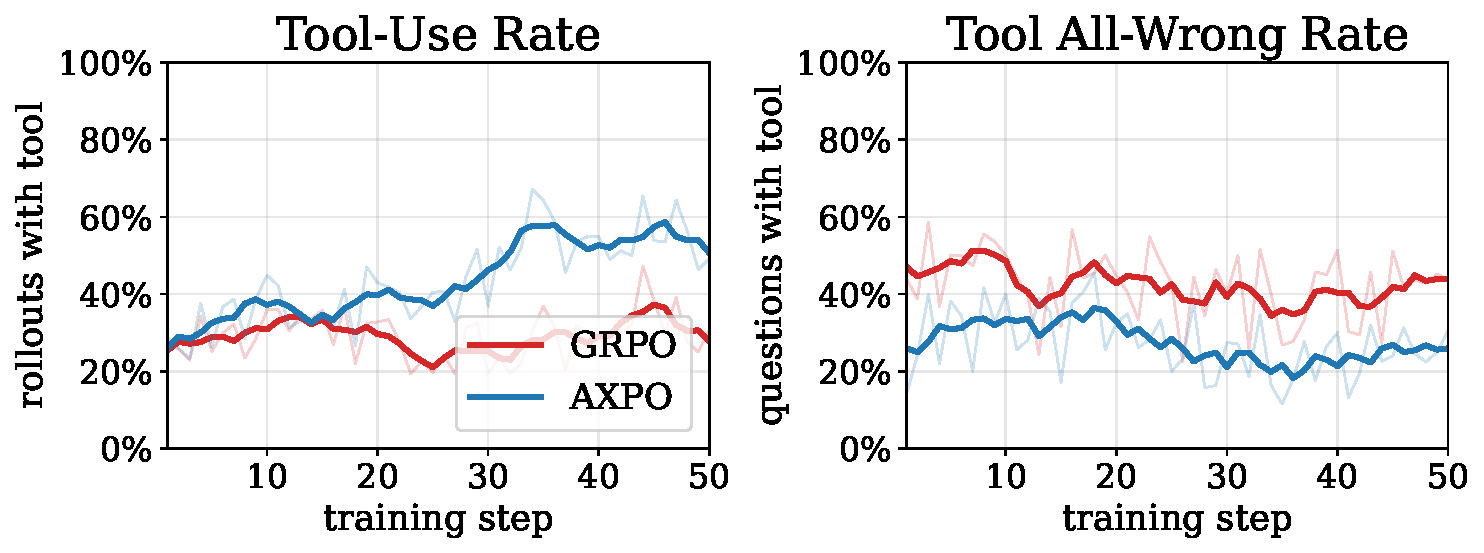
\includegraphics[width=\linewidth]{figures/fig4_training_dynamics_axpo_vs_grpo.pdf}
    \end{minipage}
    \begin{minipage}[b]{0.34\linewidth}
        \centering
        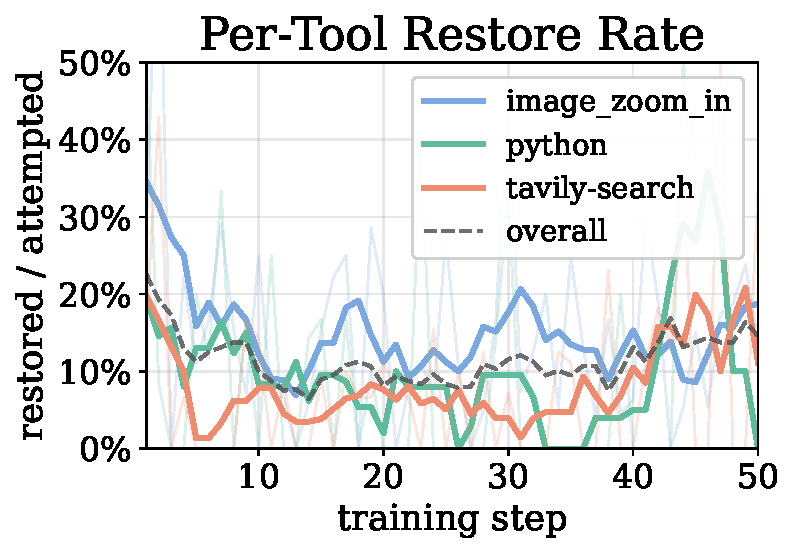
\includegraphics[width=\linewidth]{figures/fig4_per_tool_rescue.pdf}
    \end{minipage}
    \vspace{-0.1in}
    \caption{Both \gap symptoms reverse during AXPO training but stay flat under GRPO, and the recovery does happen at resampling. \textbf{Left \& Middle:} tool-use rate (top) and all-wrong rate on tool-using subgroups (bottom) over RL steps. \textbf{Right:} per-tool failed-subgroup recovery rate --- the share of all-wrong tool-using subgroups that resampling flips into a subgroup with at least one correct tool-using trajectory.}
    \vspace{-0.15in}
    \label{fig:training-dynamics}
\end{figure}

\begin{figure}[t]
    \centering
    \begin{subfigure}[b]{0.38\linewidth}
        \centering
        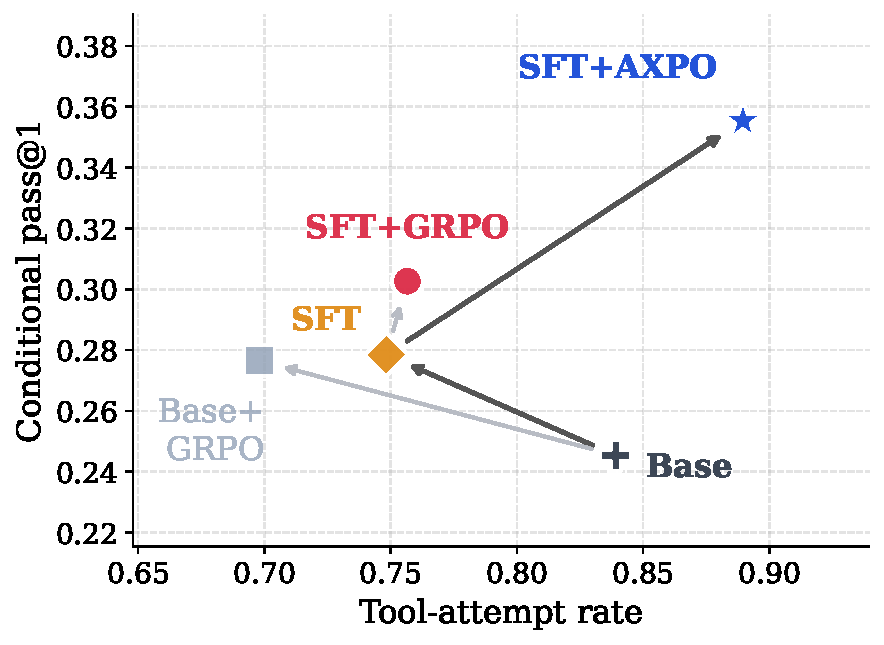
\includegraphics[width=\linewidth]{figures/figx_tool_calibration.pdf}
        \vspace{-0.15in}
        \caption{Training stages on the tool-attempt rate vs. conditional pass@1 plane. Only AXPO expands both axes simultaneously.}
        \label{fig:tool-calibration}
    \end{subfigure}\hfill
    \begin{subfigure}[b]{0.60\linewidth}
        \centering
        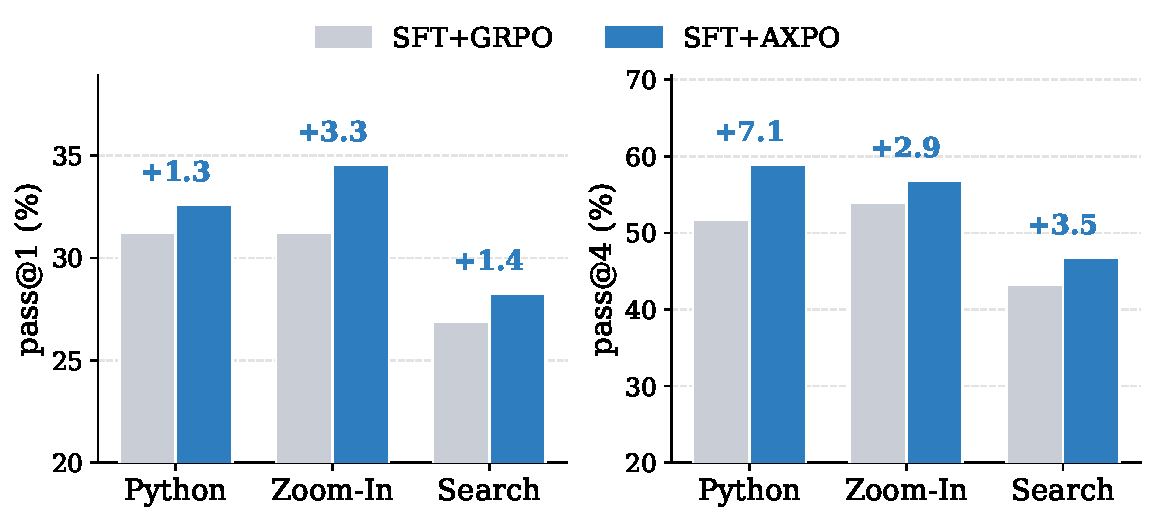
\includegraphics[width=\linewidth]{figures/figx_tool_call_quality.pdf}
        \vspace{-0.15in}
        \caption{Per-tool quality on the matched-tool-use subset (questions where both SFT+GRPO and SFT+AXPO invoke the tool). AXPO improves pass@1 and pass@4 across all three tool families.}
        \label{fig:per-tool-quality}
    \end{subfigure}
    \vspace{-0.05in}
    \caption{\textbf{Post-training analysis} pooled over MathVision, VisualProbe-Hard, and HR-MMSearch on 8B model. Conditional Pass@1 is measured on 715 tool-attempted questions from each benchmark.}
    \vspace{-0.2in}
    \label{fig:matched-analysis}
\end{figure}


\paragraph{Training dynamics.}
\autoref{fig:training-dynamics} (left \& middle) tracks the two diagnostic symptoms of \autoref{sec:gap} over RL steps. Under SFT\,+\,GRPO, the tool-use rate stays flat near $\sim$30\% and the all-wrong rate hovers around $\sim$40\% throughout training. Under SFT\,+\,AXPO, tool-use climbs $+28$\,pp over training and the all-wrong rate sits $\sim$17\,pp below GRPO at \emph{every} step, with tool-use rising during AXPO training while the all-wrong rate is suppressed by branching at each step, both consistent only under AXPO. The AXPO all-wrong rate is measured on the post-resampling subgroup composition (a tool-using subgroup that resampling recovers with at least one correct continuation no longer counts as all-wrong), so this persistent middle-panel gap is the per-step restore rate visualized in the right panel: \toolresample flips $\sim$12\% of all-wrong tool-using subgroups per step into subgroups with at least one correct tool-call continuation. This rate is non-trivial because resampling targets the hardest cases where every original tool-using rollout already failed, and restores learning signal so the policy is rewarded for tool use.

\paragraph{Test-time dynamics.}
More globally, \autoref{fig:tool-calibration} positions each training stage on the (tool-attempt rate, conditional Pass@1) plane measured on three benchmarks: every other stage either trades tool frequency for quality (Base\,$\to$\,GRPO or SFT) or holds tool frequency fixed while pushing only quality (SFT\,$\to$\,SFT\,+\,GRPO), while \textbf{only SFT\,+\,AXPO advances along both axes simultaneously}. The post-training matched-tool analysis (\autoref{fig:per-tool-quality}) is the per-question analysis of this joint advance: on questions where SFT\,+\,GRPO and SFT\,+\,AXPO both invoke a tool, AXPO improves Pass@1 across all three tool families, indicating the gain is in tool interaction quality.